\documentclass[11pt]{article}
\usepackage{tda}

\begin{document}

\section{Intro}
\label{sec:intro}

This is going to be a great document summarizing~\cite{really-great-ref}

It has some great features:

\begin{enumerate}
    \item cool math like $\N$, $\R$, $\Z$, $\S$
    \item I can reference sections with \secref{intro}
    \item I can say Bla~\etal
    \item I can say something \dave{what is going on?}
    \item I can say something \brittany{what is going on?}
    \item I can even to a todo \todo{see I have lots of cool features}
\end{enumerate}

And figures

\begin{figure}[h]
    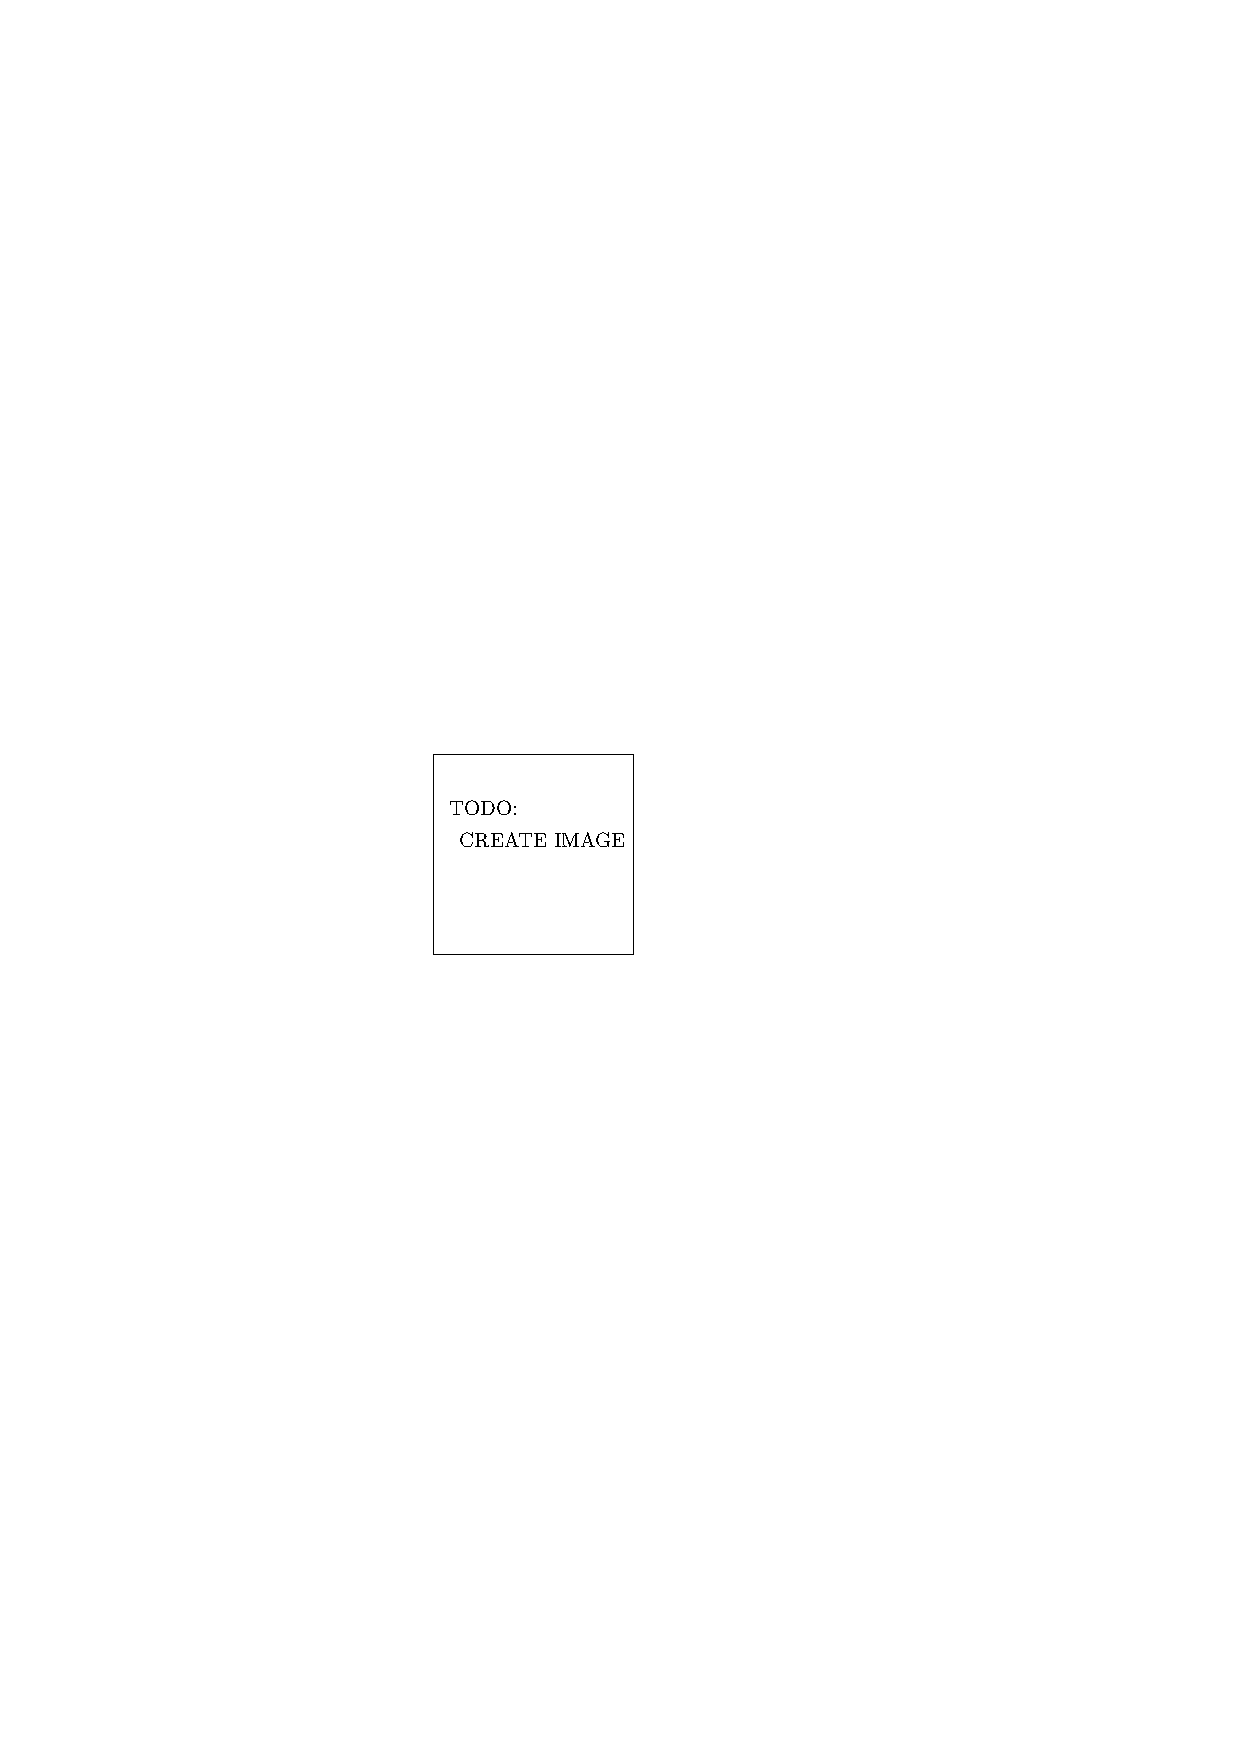
\includegraphics{todo}
    \caption{this is a todo figure}
\end{figure}

\bibliography{references}{}
\bibliographystyle{plain}
\end{document}
